% Compile:
%   pdflatex ann_primary_report.tex
% or:
%   latexmk -pdf ann_primary_report.tex
%
% Notes:
% - This document focuses on the primary model (Model 2): ANN with categorical embeddings + MLP.
% - For an overall comparison across all models, see `REPORT.md` and `report.tex`.
% - For interactive plots with one-click PNG/SVG downloads, open `plots/report_graphs.html`.

\documentclass[11pt]{article}

\usepackage[margin=1in]{geometry}
\usepackage{microtype}
\usepackage{amsmath}
\usepackage{booktabs}
\usepackage{graphicx}
\usepackage{siunitx}
\usepackage{enumitem}
\usepackage{xcolor}
\usepackage{hyperref}
\usepackage{pgfplots}
\usepackage{subcaption}
\usepackage{tabularx}
\usepackage{array}
\usepackage{listings}
\usepackage{tikz}
\usetikzlibrary{positioning,arrows.meta}

\pgfplotsset{compat=1.18}
\sisetup{detect-weight=true, detect-family=true}
\hypersetup{
  colorlinks=true,
  linkcolor=blue!60!black,
  urlcolor=blue!60!black,
  citecolor=blue!60!black
}

\lstset{
  basicstyle=\ttfamily\small,
  breaklines=true,
  columns=fullflexible,
  frame=single,
  framerule=0.3pt,
  rulecolor=\color{black!20},
  upquote=true
}

% -----------------------------
% Key numbers (copied from results_all.csv / eval_suite as of 2026-03-12)
% -----------------------------
\newcommand{\NTotal}{597{,}928}
\newcommand{\NTrain}{418{,}549}
\newcommand{\NVal}{89{,}689}
\newcommand{\NTest}{89{,}690}

% Primary model config (full features)
\newcommand{\AnnHidden}{\texttt{512→256→128→64}}
\newcommand{\AnnDropout}{0.10}
\newcommand{\AnnEmbedCap}{64}
\newcommand{\AnnEpochs}{30}
\newcommand{\AnnBatch}{512}
\newcommand{\AnnLR}{0.004}
\newcommand{\AnnWD}{0.001}
\newcommand{\AnnParams}{629{,}340}
\newcommand{\AnnEmbParams}{346{,}203}
\newcommand{\AnnMlpParams}{283{,}137}

% Best checkpoint metrics (seed=42, split_seed=42, random split)
\newcommand{\AnnBestEpoch}{28}
\newcommand{\AnnBestTrainRmse}{0.1265}
\newcommand{\AnnBestValRmse}{0.1388}
\newcommand{\AnnBestTestRmse}{0.1433}
\newcommand{\AnnBestTrainAcc}{93.06}
\newcommand{\AnnBestValAcc}{92.67}
\newcommand{\AnnBestTestAcc}{92.62}

% Last-epoch metrics (overfitting signal)
\newcommand{\AnnLastValRmse}{0.1399}
\newcommand{\AnnLastTestRmse}{0.1439}
\newcommand{\AnnLastValAcc}{92.49}
\newcommand{\AnnLastTestAcc}{92.39}

% Robustness (eval_suite; mean ± std)
\newcommand{\AnnRandRmseMean}{0.1420}
\newcommand{\AnnRandRmseStd}{0.0036}
\newcommand{\AnnRandAccMean}{92.64}
\newcommand{\AnnRandAccStd}{0.31}
\newcommand{\AnnTimeRmseMean}{0.3146}
\newcommand{\AnnTimeRmseStd}{0.0365}
\newcommand{\AnnTimeAccMean}{82.78}
\newcommand{\AnnTimeAccStd}{2.35}

% -----------------------------
% Plot data blocks (generated from the best ANN run; seed=42, split_seed=42)
% -----------------------------
\pgfplotstableread[col sep=space]{
epoch valrmse
1 0.450544
2 0.466490
3 0.577868
4 0.348379
5 0.200257
6 0.195003
7 0.180563
8 0.204513
9 0.166933
10 0.162415
11 0.165542
12 0.161614
13 0.153863
14 0.152829
15 0.148012
16 0.153378
17 0.145649
18 0.144533
19 0.145887
20 0.148402
21 0.147381
22 0.144280
23 0.151947
24 0.145088
25 0.143164
26 0.148880
27 0.144925
28 0.138833
29 0.141125
30 0.139866
}\AnnValCurve

\pgfplotstableread[col sep=space]{
true pred
12.490879 12.637133
13.847011 13.732607
12.691584 12.946992
12.691584 12.607306
13.253391 13.254912
12.886643 13.015642
12.724870 12.843979
13.102162 13.223688
13.180634 13.267639
14.169683 14.019829
13.377007 13.371414
13.326122 13.294516
13.083625 12.907050
13.191892 13.070986
13.641158 13.634086
14.220976 14.222865
12.925134 13.001558
13.977631 14.088026
12.644009 12.638067
13.371566 13.315630
13.285844 13.378147
12.574185 12.645528
13.672795 13.779134
13.060490 13.076858
13.272508 13.208745
12.861001 12.643908
13.199327 13.181545
12.314932 12.392358
13.355062 13.338869
12.611541 12.823874
12.971542 13.194136
12.736704 12.706965
13.660027 13.629684
13.997833 13.765585
13.399997 13.374342
13.256896 13.342581
12.278398 12.365957
13.790194 13.574777
13.102162 13.136698
12.858400 12.963454
13.217675 13.203879
13.199327 13.090696
12.983104 13.026800
13.258643 13.319352
13.407544 13.446483
14.006132 13.812953
13.282782 12.990695
13.190023 13.146706
13.130334 13.127965
13.687565 13.858587
12.861521 12.910637
14.508658 13.971517
13.171155 13.418289
13.710151 13.729688
12.487489 12.583721
13.588612 13.625209
12.100718 12.356492
14.331325 14.390392
13.017005 13.189884
13.662360 13.776839
13.761055 13.820518
13.873780 13.812468
13.759999 13.847028
13.353477 13.529911
13.253393 13.190769
14.139404 13.715511
12.598118 12.479633
14.042647 13.971017
13.226726 13.278860
13.242811 13.338018
13.270785 13.272878
12.459167 12.791162
13.560619 13.324937
13.534474 13.615018
13.892472 13.881107
13.473022 14.091394
13.487008 13.152095
12.542548 12.627871
13.465955 13.433639
13.161586 13.151710
13.551546 13.455865
13.089842 13.323921
13.803439 13.724523
13.413124 13.284705
13.190023 13.273765
13.038984 13.142634
13.652993 13.604478
12.847929 12.971486
13.122365 13.133651
13.662360 13.645332
13.081544 13.095240
13.592368 13.788304
13.774690 13.806740
13.262127 13.046497
13.312985 13.290083
13.346308 13.343227
12.254868 12.358297
13.164467 13.165952
13.795309 13.714266
13.748302 13.765908
14.169683 14.199930
12.840003 12.632563
13.399845 13.279055
13.635188 13.669043
12.730804 12.880669
13.407544 13.400270
13.602443 13.543346
13.412045 13.329273
12.911645 12.981752
13.357595 13.342173
13.748302 13.792490
12.818555 12.921290
12.963370 12.988853
12.943215 13.061891
12.873904 13.220230
13.441545 13.319860
12.914111 12.990220
13.550243 13.482666
12.594734 12.666965
13.279368 13.296596
}\AnnPredScatter

\pgfplotstableread[col sep=space]{
center count
-0.966667 5
-0.900000 13
-0.833333 15
-0.766667 17
-0.700000 24
-0.633333 48
-0.566667 90
-0.500000 168
-0.433333 290
-0.366667 537
-0.300000 1040
-0.233333 2222
-0.166667 4600
-0.100000 9946
-0.033333 18526
0.033333 22823
0.100000 15840
0.166667 7548
0.233333 3202
0.300000 1362
0.366667 633
0.433333 316
0.500000 137
0.566667 74
0.633333 68
0.700000 34
0.766667 27
0.833333 11
0.900000 7
0.966667 8
}\AnnResidHist

\pgfplotstableread[col sep=space]{
year acc
2009 90.895
2010 91.832
2011 92.273
2012 92.866
2013 92.709
2014 92.736
2015 93.037
2016 92.783
2017 92.216
2018 92.996
2019 93.275
}\AnnYearAcc

\pgfplotstableread[col sep=space]{
decile acc mdape lo hi n
1 88.538 0.114623 10000 300000 8809
2 92.213 0.077871 300000 372000 9110
3 93.342 0.066581 372000 434000 8951
4 94.181 0.058193 434000 496000 8971
5 93.716 0.062839 496000 568000 8965
6 94.392 0.056084 568000 648000 8966
7 93.541 0.064595 648000 743590 9011
8 92.612 0.073882 743590 880000 8939
9 91.813 0.081871 880000 1190000 8984
10 88.474 0.115257 1190000 22000005 8984
}\AnnDecileAcc

\title{Primary Model: ANN (Categorical Embeddings + MLP)\\
\large Architecture, Complexity, and Results}
\author{RPSAps360 Project}
\date{March 12, 2026}

\begin{document}
\maketitle

\begin{abstract}
This document describes the current primary model for predicting \texttt{TransactionPrice}: an artificial neural network (ANN) that combines standardized numeric features with learned embeddings for high-cardinality categorical features, followed by a multilayer perceptron (MLP). We provide an architecture diagram, parameter counts, reproducible hyperparameters, and both quantitative and qualitative evaluation results. Canonical results are tracked in a single CSV (\texttt{results\_all.csv}); an offline dashboard (\texttt{plots/report\_graphs.html}) provides one-click PNG/SVG downloads of plots.
\end{abstract}

\tableofcontents
\newpage

\section{Model choice and rationale}
\paragraph{Why an embedding-based ANN makes sense for this dataset.}
The dataset includes multiple high-cardinality categorical variables (e.g.\ \texttt{PropertyStyle}, \texttt{PropertyUse}) alongside numeric variables (e.g.\ \texttt{LivingArea}, \texttt{YearBuilt}, lat/lon). One-hot encoding would create an extremely wide feature vector. Instead, the ANN learns a compact embedding vector per categorical column and concatenates all embeddings with standardized numeric features, allowing the MLP to learn nonlinearities and interactions (size \(\times\) location, time trends by neighborhood, etc.).

\section{Architecture (diagram + complexity)}
\subsection{High-level diagram}
\begin{figure}[h]
\centering
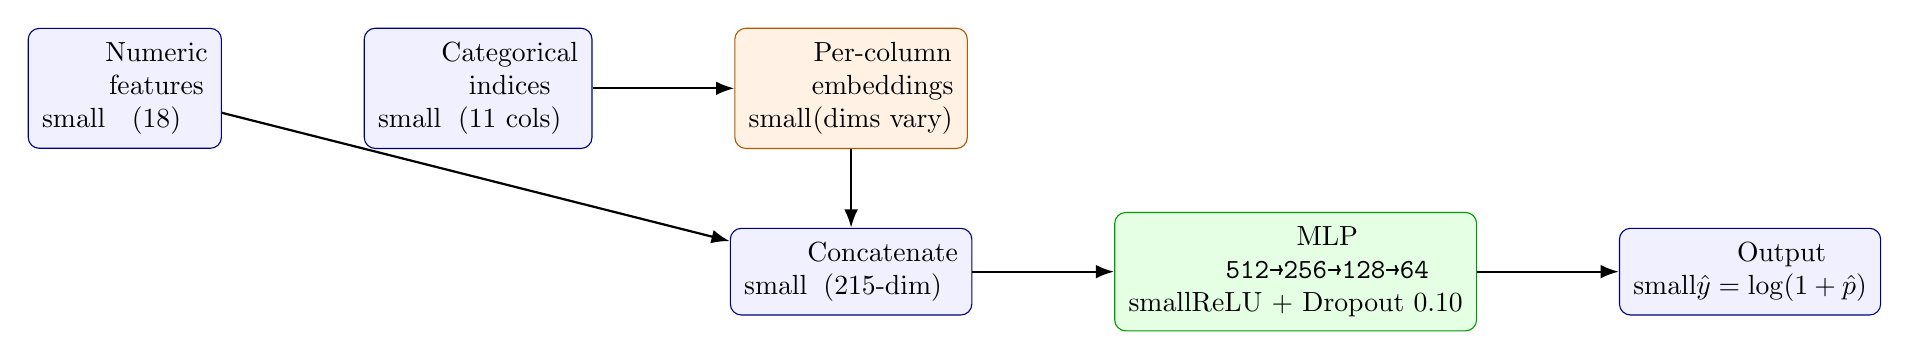
\begin{tikzpicture}[
  node/.style={draw, rounded corners, align=center, inner sep=5pt, font=\\small},
  arrow/.style={-Latex, thick},
  box/.style={node, fill=blue!6, draw=blue!50!black},
  emb/.style={node, fill=orange!10, draw=orange!70!black},
  mlp/.style={node, fill=green!10, draw=green!60!black}
]
\node[box] (num) {Numeric\\features\\(\(18\))};
\node[box, right=18mm of num] (cat) {Categorical\\indices\\(\(11\) cols)};
\node[emb, right=18mm of cat] (embs) {Per-column\\embeddings\\(dims vary)};
\node[box, below=10mm of embs] (concat) {Concatenate\\(215-dim)};
\node[mlp, right=18mm of concat] (mlp1) {MLP\\\AnnHidden\\ReLU + Dropout \AnnDropout};
\node[box, right=18mm of mlp1] (out) {Output\\\(\hat{y}=\log(1+\hat{p})\)};

\draw[arrow] (num) -- (concat);
\draw[arrow] (cat) -- (embs);
\draw[arrow] (embs) -- (concat);
\draw[arrow] (concat) -- (mlp1);
\draw[arrow] (mlp1) -- (out);
\end{tikzpicture}
\caption{Primary model architecture (ANN with categorical embeddings + MLP).}
\label{fig:ann-arch}
\end{figure}

\subsection{Parameter count and layer sizes}
The best-performing full-feature ANN uses:
\begin{itemize}[leftmargin=*]
  \item \textbf{Input:} 18 standardized numeric features + 11 categorical embedding vectors (total concatenated dimension \(=215\)).
  \item \textbf{Hidden layers:} \AnnHidden\ (4 hidden layers, ReLU activations).
  \item \textbf{Regularization:} dropout \(\approx\)\AnnDropout\ and weight decay \(\approx\)\AnnWD.
  \item \textbf{Total parameters:} \AnnParams\ (\AnnEmbParams\ in embeddings, \AnnMlpParams\ in the MLP).
\end{itemize}

\begin{table}[h]
\centering
\small
\begin{tabular}{@{}lrrr@{}}
\toprule
Categorical column & Categories & Emb dim & Parameters \\
\midrule
\texttt{BuildingType} & 995 & 32 & 31{,}840 \\
\texttt{PropertyStyle} & 3{,}356 & 58 & 194{,}648 \\
\texttt{Condition} & 8 & 4 & 32 \\
\texttt{FSA} & 234 & 16 & 3{,}744 \\
\texttt{gcode\_City} & 325 & 19 & 6{,}175 \\
\texttt{Basement} & 6 & 4 & 24 \\
\texttt{Parking\_Type} & 8 & 4 & 32 \\
\texttt{Ownership} & 5 & 4 & 20 \\
\texttt{PropertyUse} & 2{,}284 & 48 & 109{,}632 \\
\texttt{BRPS\_Style} & 9 & 4 & 36 \\
\texttt{gcode\_MatchStatus} & 5 & 4 & 20 \\
\bottomrule
\end{tabular}
\caption{Embedding table sizes for the full feature set. Embedding dimensions follow the rule in \texttt{train\_ann.py}: \(\min(\texttt{embed\_dim\_cap},\max(4,\lfloor \sqrt{\text{cat\_size}}\rfloor + 1))\).}
\label{tab:ann-embeddings}
\end{table}

\section{Training setup (reproducible details)}
\subsection{Target and loss}
\begin{itemize}[leftmargin=*]
  \item \textbf{Target:} \(y=\log(1+\texttt{TransactionPrice})\) (stored as \texttt{y\_log1p}).
  \item \textbf{Loss:} mean squared error in log space.
  \item \textbf{Optimizer:} AdamW (\(\texttt{lr}=\AnnLR\), \(\texttt{weight\_decay}=\AnnWD\)).
  \item \textbf{Checkpointing:} keep the epoch with lowest validation MSE (best checkpoint).
\end{itemize}

\subsection{Splits}
All experiments use the same dataset size (\NTotal) and a 70/15/15 split:
\begin{itemize}[leftmargin=*]
  \item \textbf{Random split:} \NTrain/\NVal/\NTest with a fixed \texttt{split\_seed}.
  \item \textbf{Time split:} train on earlier (\texttt{TransactionYear}, \texttt{Quarter}) and test on later transactions (\texttt{--split-strategy time}).
\end{itemize}

\subsection{Metrics}
We report:
\begin{itemize}[leftmargin=*]
  \item \textbf{RMSE(log):} RMSE on \(\log(1+\text{price})\) (lower is better).
  \item \textbf{Accuracy \%:} derived from price-space MdAPE: \(\max(0, 100\cdot(1-\text{MdAPE}))\) (higher is better).
\end{itemize}

\section{Quantitative results (feasibility)}
\subsection{Best single run (full features; random split)}
The best recorded run (seed=42, split\_seed=42) achieves:
\begin{itemize}[leftmargin=*]
  \item \textbf{Test RMSE(log):} \AnnBestTestRmse
  \item \textbf{Test accuracy:} \AnnBestTestAcc\%
  \item \textbf{Best checkpoint epoch:} \AnnBestEpoch\ (out of \AnnEpochs)
\end{itemize}

\begin{table}[h]
\centering
\small
\begin{tabular}{@{}lrrr@{}}
\toprule
Checkpoint & Train & Validation & Test \\
\midrule
\textbf{Best (epoch \AnnBestEpoch)} RMSE(log) & \AnnBestTrainRmse & \AnnBestValRmse & \AnnBestTestRmse \\
\textbf{Best (epoch \AnnBestEpoch)} Accuracy (\%) & \AnnBestTrainAcc & \AnnBestValAcc & \AnnBestTestAcc \\
\addlinespace
\textbf{Last (epoch \AnnEpochs)} RMSE(log) & --- & \AnnLastValRmse & \AnnLastTestRmse \\
\textbf{Last (epoch \AnnEpochs)} Accuracy (\%) & --- & \AnnLastValAcc & \AnnLastTestAcc \\
\bottomrule
\end{tabular}
\caption{Best vs last checkpoint. The small drop from best to last illustrates mild overfitting; the best checkpoint is selected by validation MSE.}
\label{tab:ann-best-vs-last}
\end{table}

\subsection{Robustness across random seeds and data splits}
To verify the improvement is not due to a favorable split, the best ANN config is rerun across multiple random split seeds and model seeds (\texttt{eval\_suite.py}; logged in \texttt{results\_all.csv}).
\begin{itemize}[leftmargin=*]
  \item \textbf{Random split (21 runs):} test RMSE(log) \AnnRandRmseMean\(\pm\)\AnnRandRmseStd; test accuracy \AnnRandAccMean\(\pm\)\AnnRandAccStd\%.
  \item \textbf{Time split (9 runs):} test RMSE(log) \AnnTimeRmseMean\(\pm\)\AnnTimeRmseStd; test accuracy \AnnTimeAccMean\(\pm\)\AnnTimeAccStd\%.
\end{itemize}

\section{Qualitative and diagnostic results}
\subsection{Learning curve (validation RMSE)}
\begin{figure}[h]
\centering
\begin{tikzpicture}
\begin{axis}[
  xlabel={Epoch},
  ylabel={Validation RMSE(log)},
  xmin=1, xmax=30,
  ymin=0.13, ymax=0.60,
  ymajorgrids=true,
  xmajorgrids=true,
]
\addplot+[mark=*, mark size=1.0pt, color=blue!70!black] table[x=epoch,y=valrmse] {\AnnValCurve};
\addplot+[only marks, mark=star, mark size=2.0pt, color=red!70!black] coordinates {(\AnnBestEpoch,\AnnBestValRmse)};
\end{axis}
\end{tikzpicture}
\caption{Validation learning curve (RMSE in log space). Best checkpoint occurs at epoch \AnnBestEpoch.}
\label{fig:ann-val-curve}
\end{figure}

\subsection{Prediction scatter and residual distribution (test set)}
\begin{figure}[h]
\centering
\begin{subfigure}{0.49\linewidth}
\centering
\begin{tikzpicture}
\begin{axis}[
  xlabel={True log1p(price)},
  ylabel={Predicted log1p(price)},
  xmin=11.0, xmax=16.0,
  ymin=11.0, ymax=16.0,
  grid=both,
  legend style={at={(0.02,0.98)},anchor=north west},
]
\addplot+[only marks, mark=o, mark size=1.4pt, color=blue!60!black] table[x=true,y=pred] {\AnnPredScatter};
\addlegendentry{ANN (sample)}
\addplot+[domain=11:16, samples=2, color=black!60] {x};
\addlegendentry{Ideal y=x}
\end{axis}
\end{tikzpicture}
\caption{Predicted vs true (120 sampled test points).}
\end{subfigure}
\hfill
\begin{subfigure}{0.49\linewidth}
\centering
\begin{tikzpicture}
\begin{axis}[
  ybar,
  bar width=6pt,
  xlabel={Residual (pred\_log − true\_log)},
  ylabel={Count},
  xmin=-1.05, xmax=1.05,
  ymajorgrids=true,
]
\addplot+[fill=blue!18, draw=blue!60!black] table[x=center,y=count] {\AnnResidHist};
\end{axis}
\end{tikzpicture}
\caption{Residual histogram (test set).}
\end{subfigure}
\caption{Qualitative plots for the primary ANN (best checkpoint).}
\label{fig:ann-qual}
\end{figure}

\subsection{Performance on classes of samples}
\begin{figure}[h]
\centering
\begin{subfigure}{0.49\linewidth}
\centering
\begin{tikzpicture}
\begin{axis}[
  xlabel={TransactionYear},
  ylabel={Test accuracy (\%)},
  ymin=88, ymax=94,
  ymajorgrids=true,
  xmajorgrids=true,
]
\addplot+[mark=*, color=green!60!black] table[x=year,y=acc] {\AnnYearAcc};
\end{axis}
\end{tikzpicture}
\caption{Accuracy by year (test set).}
\end{subfigure}
\hfill
\begin{subfigure}{0.49\linewidth}
\centering
\begin{tikzpicture}
\begin{axis}[
  xlabel={True-price decile (test set)},
  ylabel={Test accuracy (\%)},
  ymin=86, ymax=95,
  ymajorgrids=true,
  xmajorgrids=true,
]
\addplot+[mark=*, color=purple!70!black] table[x=decile,y=acc] {\AnnDecileAcc};
\end{axis}
\end{tikzpicture}
\caption{Accuracy by true-price decile. Extremes (lowest/highest deciles) are harder.}
\end{subfigure}
\caption{Qualitative breakdowns: model behavior differs across subgroups of the data.}
\label{fig:ann-subgroups}
\end{figure}

\subsection{Selected examples (price-space errors)}
\begin{table}[h]
\centering
\small
\begin{tabularx}{\linewidth}{@{}lrrrr>{\raggedright\arraybackslash}X@{}}
\toprule
Example & True price & Pred price & APE (\%) & Year & Context (FSA / City) \\
\midrule
\textbf{p5 (very accurate)} & \$1{,}020{,}000 & \$1{,}026{,}681 & 0.66 & 2015 & \texttt{M3H} / TORONTO \\
\textbf{p50 (typical)} & \$797{,}900 & \$738{,}979 & 7.38 & 2013 & \texttt{L4C} / RICHMOND HILL \\
\textbf{p95 (large error)} & \$260{,}000 & \$334{,}129 & 28.51 & 2013 & \texttt{L6T} / BRAMPTON \\
\bottomrule
\end{tabularx}
\caption{Three representative test samples from the best-checkpoint model, chosen by APE percentiles (5th/50th/95th). This provides a qualitative sense of typical vs worst-case behavior.}
\label{tab:ann-examples}
\end{table}

\section{Challenges and limitations}
\begin{itemize}[leftmargin=*]
  \item \textbf{High-cardinality categoricals:} embedding tables are essential to avoid impractically wide one-hot vectors.
  \item \textbf{Missingness + sentinels:} the pipeline normalizes tokens like \texttt{NA}/\texttt{NULL}/\texttt{-999}; inconsistent missing codes are a recurring data-engineering challenge.
  \item \textbf{Time generalization:} random splits mix years; time splits are needed to test forward-looking generalization (performance drops but remains strong relative to linear baselines).
  \item \textbf{Preprocessing leakage:} the current tensorization computes normalization/vocab on the full dataset (simpler but slightly optimistic); a stricter version would compute these on training data only per split.
\end{itemize}

\section{Reproduction commands}
\subsection{Train the primary ANN (best known config)}
\begin{lstlisting}[language=bash]
python train_ann.py --data ann_tensors_full.pt --split-strategy random --seed 42 \
  --epochs 30 --batch-size 512 --lr 0.004 --weight-decay 0.001 \
  --hidden-dims 512,256,128,64 --dropout 0.1 --embed-dim-cap 64 \
  --out-csv ann_runs.csv --run-name full_deep4_bs512_lr4e-3_do0.1_wd1e-3

python export_results.py   # merges into results_all.csv
\end{lstlisting}

\subsection{Robustness checks (multi-seed, random + time splits)}
\begin{lstlisting}[language=bash]
python eval_suite.py --data ann_tensors_full.pt --models ann,hedonic \
  --split-strategies random,time --split-seeds 42,7,123 --model-seeds 0,1,42 \
  --out-csv eval_runs.csv

python export_results.py
\end{lstlisting}

\subsection{Downloadable graph pack}
\begin{lstlisting}[language=bash]
python make_report_graphs.py --results results_all.csv --out plots/report_graphs.html
\end{lstlisting}

\end{document}
